\documentclass[final,onecolumn]{elsarticle}
\usepackage{amssymb}
\usepackage{amsmath}
\usepackage{pgfplots}
\pgfplotsset{compat=1.14}
\usepackage{tikz,pgfplots}
\usetikzlibrary{shapes,arrows,calc}
\usetikzlibrary{arrows, decorations.markings}

\begin{document}

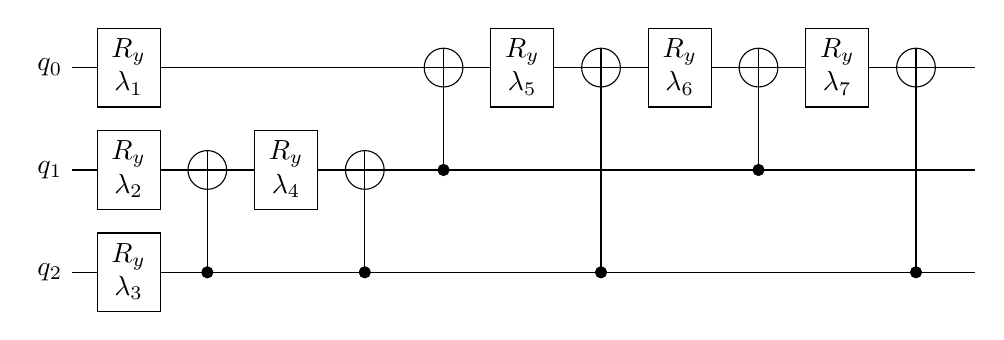
\begin{tikzpicture}[object/.style={thin,double,<->}]
\draw (0,0) -- (11.75,0);
\draw (0,-1.3) -- (11.75,-1.3);
\draw (0,-2.6) -- (11.75,-2.6);
\node at (0,0) [rectangle,draw=white ,fill=white] {$q_0$};
\node at (0,-1.3) [rectangle,draw=white ,fill=white] {$q_1$};
\node at (0,-2.6) [rectangle,draw=white ,fill=white] {$q_2$};
\draw (1,0) node[minimum height=1cm,minimum width=0.8cm, fill=white,draw] {};
\node at (1,-0.2) [rectangle,draw=none ,fill=none] {$\lambda_1$};
\node at (1,0.2) [rectangle,draw=none ,fill=none] {$R_y$};
\draw (1,-1.3) node[minimum height=1cm,minimum width=0.8cm, fill=white,draw] {};
\node at (1,-1.5) [rectangle,draw=none ,fill=none] {$\lambda_2$};
\node at (1,-1.1) [rectangle,draw=none ,fill=none] {$R_y$};
\draw (1,-2.6) node[minimum height=1cm,minimum width=0.8cm, fill=white,draw] {};
\node at (1,-2.8) [rectangle,draw=none ,fill=none] {$\lambda_3$};
\node at (1,-2.4) [rectangle,draw=none ,fill=none] {$R_y$};
\filldraw[black] (2,-2.6) circle (2pt);
\draw (2,-1.3) circle [radius=7pt];
\draw (2,-1.05) -- (2,-2.6);
\draw (3,-1.3) node[minimum height=1cm,minimum width=0.8cm, fill=white,draw] {};
\node at (3,-1.5) [rectangle,draw=none ,fill=none] {$\lambda_4$};
\node at (3,-1.1) [rectangle,draw=none ,fill=none] {$R_y$};
\filldraw[black] (4,-2.6) circle (2pt);
\draw (4,-1.3) circle [radius=7pt];
\draw (4,-1.05) -- (4,-2.6);
\filldraw[black] (5,-1.3) circle (2pt);
\draw (5,0) circle [radius=7pt];
\draw (5,0.25) -- (5,-1.3);
\draw (6,0) node[minimum height=1cm,minimum width=0.8cm, fill=white,draw] {};
\node at (6,-0.2) [rectangle,draw=none ,fill=none] {$\lambda_5$};
\node at (6,0.2) [rectangle,draw=none ,fill=none] {$R_y$};
\filldraw[black] (7,-2.6) circle (2pt);
\draw (7,0) circle [radius=7pt];
\draw (7,0.25) -- (7,-2.6);
\draw (8,0) node[minimum height=1cm,minimum width=0.8cm, fill=white,draw] {};
\node at (8,-0.2) [rectangle,draw=none ,fill=none] {$\lambda_6$};
\node at (8,0.2) [rectangle,draw=none ,fill=none] {$R_y$};
\filldraw[black] (9,-1.3) circle (2pt);
\draw (9,0) circle [radius=7pt];
\draw (9,0.25) -- (9,-1.3);
\draw (10,0) node[minimum height=1cm,minimum width=0.8cm, fill=white,draw] {};
\node at (10,-0.2) [rectangle,draw=none ,fill=none] {$\lambda_7$};
\node at (10,0.2) [rectangle,draw=none ,fill=none] {$R_y$};
\filldraw[black] (11,-2.6) circle (2pt);
\draw (11,0) circle [radius=7pt];
\draw (11,0.25) -- (11,-2.6);
\end{tikzpicture}

\end{document}